
In applications, e.g. the model studied in \Cref{cha:analysis_of_selected_models}, we are interested in the performance of the importance sampling proposals generated by the \gls{la}, \gls{cem} and \gls{eis} under more complex circumstances than those discussed in \Cref{ex:univ-gaussian-mu-fixed,ex:univ-gaussian-s2-fixed}. In particular, the dimension of $\psi$ is high ($\mathcal O(n \cdot m)$ or even $\mathcal O(n \cdot m^{2})$) and proposals may not come from a natural exponential family, so analysis based on \Cref{thm:cem-clt,thm:eis-clt} is not possible. \todo{really?} Instead, we resort to simulation studies to gain insights into the circumstances when one should prefer one method over the other.
As a leading example, we will use the following vector-autoregressive state space model with negative binomial observations. A similar, though more involved, model is studied in \Cref{sec:regional_growth_factor_model} with real data.

\begin{example}[Negative Binomial $\operatorname{VAR}(1)$ \gls{ssm}]
    \label{ex:negbinom-ar1}
    % setup 
    In this example, we consider a \gls{ssm} where states $X_{t}$ follow a stationary Gaussian $\operatorname{VAR}(1)$ process, initialized in its stationary distribution $\mathcal N(0,\Sigma)$ for \acrshort{spd} $\Sigma$. For simplicity let the transition matrices be given by a multiple of the identity, i.e. $A_{t} = \alpha I_{m}$ for all $t$ where $\alpha \in (-1, 1)$
    In total, the states are governed by
    \begin{align*}
    X_{0} &\sim \mathcal N(0,\Sigma) \\
    X_{t} &= \alpha X_{t - 1} + \varepsilon_{t}\\
    \varepsilon_t &\iid \mathcal N(0, (1 - \alpha^{2})\Sigma), t = 1, \dots, n
    \end{align*}
    where the $\varepsilon_{1}, \dots, n$ and $X_{0}$ are jointly independent. The observations follow a conditional negative binomial distribution 
    $$
    Y^{i}_{t} | X_{t} \sim \nbinom \left( \exp(X^{i}_{t}), r \right), \phantom{and} i = 1, \dots, p \phantom{and} t = 0, \dots, n
    $$
    and individual observations are conditionally independent given the current state. The parametrization of the negative binomial distribution $\nbinom \left( \mu, r \right)$ is such that the density is
    $$
        p_{\mu, r}(y) = \binom{y + r - 1}{r} \left( \frac{\mu}{r + \mu} \right)^{y} \left( \frac{r}{r + \mu} \right)^{r} \propto \mu^{y} (\mu + r)^{-(r + y)},
    $$
    where proportionality is in $\mu$, with expectation $\mu$, variance $\mu + \frac{\mu^{2}}{r}$ and support $\N_{0}$. 
\end{example}

%% simulation study on MSE/Bias/Variance

Our first simulation study concerns the non-asymptotic behavior of the \gls{cem} and \gls{eis} estimators, i.e. finite sample analogs of \Cref{thm:cem-clt,thm:eis-clt}. To this end,
we let $m = 1$ in \Cref{ex:negbinom-ar1}, fix $n$ to $100$ and set $\Sigma = \sigma^{2} = 1$. 
We then simulate once from the marginal distribution of $Y$ and perform the \gls{la} to a prespecified precision $\epsilon$ and maximum number of iterations $n_{\text{iter}}$, obtaining a proposal distribution $\G_{\la}$. Using a large number of samples $N_{\text{true}}$ from this proposal we find the optimal $\G_{\ce}$ and $\G_{\eis}$ using the same desired precision and number of iterations as for the \gls{la}. For the remainder of this section, we ignore sampling variation in these proposals and treat them as exact. 

%% posterior marginal means and variances
To determine the non-asymptotic sampling behavior we now perform the above procedure again, using only $N \ll N_{\text{true}}$ many samples for both procedures, obtaining proposals $\hat\P^{N}_{\ce}$ and $\hat \P^{N}_{\eis}$. The full proposals are Gaussian distributions on $\R^{(n+1)\times m}$, either given as the posterior of a \gls{glssm} (\gls{la}, \gls{eis}) or by a Gaussian Markov process(\gls{cem}), see \Cref{sec:gaussian_importance_sampling_for_state_space_models}. 
This procedure is repeated $M$ times for every sample size $N$ considered, with different initial random seeds, obtaining $\hat\P^{N,i}_{\ce}$ and $\hat \P^{N,i}_{\eis}$ for $i = 1, \dots, M$.

To assess the speed of convergence of the \gls{cem} and \gls{eis} we then estimate the mean squared error of means and variances of the $(n+1) \times m$ univariate marginals as $N$, the number of samples used to obtain $\hpce$ or $\hpeis$, grows. For the true value, we take the univariate means and variances of $\G_{\ce}$ and $\G_{\eis}$ respectively. Additionally, we perform a bias-variance decomposition to see where the estimation error originates. 

More concretely, fix $N$ and denote by $\mu, \sigma^{2} \in \mathbf R^{(n + 1) \cdot m}$ the marginal means and variances of $\G_{\ce}$ ($\G_{\eis}$). 
Let $\hat\mu_{i}, \hat\sigma^{2}_{i}\in\mathbf R^{(n + 1) \cdot m}$ be the marginal means and variances of $\G^{N,i}_{\ce}$ ($\G^{N,i}_{\eis}$) for $i = 1,\dots, M$. 
Now 
$$
\widehat{\text{aMSE}} = \frac{1}{M} \frac{1}{(n + 1)m} \sum_{i = 1}^M \lVert \mu - \hat\mu_{i} \rVert_{2}^2 + \lVert \sigma^{2} - \hat\sigma_{i}^2 \rVert^{2}_{2}
$$
is an estimate of the mean-squared error of $(\mu, \sigma^{2})$, where we divide by $(n+1)m$ to make estimates comparable across models of different dimensions. 

%The $\text{ASE}_{i}$ is of interest to the practitioner as they usually only run a single iteration of the optimal importance sampling procedure. So while a low $\text{AMSE}$ is desirable, the variance of $\text{ASE}$ should also be small in practice, as otherwise several runs of the optimal importance sampling procedure may be required to obtain a good proposal.

In \Cref{fig:mse_bias_var_decomposition} we show the $\widehat{\text{aMSE}}$ for both the \gls{cem} and \gls{eis} for varying values of $N$. As is evident from this Figure, the \gls{cem} consistently has a larger aMSE than \gls{eis}, for all values of $N$. Thus the \gls{cem} requires several orders of magnitude more samples to obtain the same precision as \gls{eis}.

For further investigation, we perform a bias-variance decomposition of the aMSE for both the means $\mu$ and variances $\sigma^{2}$. Consider the average means and variances over the $M$ simulations,
\begin{align*}
    \bar \mu = \frac{1}{M} \sum_{i=1}^{M} \hat\mu_{i} && \bar \sigma^{2} = \frac{1}{M} \sum_{i=1}^{M} \hat\sigma^{2}_{i},
\end{align*}
and the state-average squared bias and variance
\begin{align*}
    \text{aBias}^{2}_{\mu} &= \frac{1}{(n+1)m} \lVert \mu - \bar\mu \rVert^{2}_{2}, \\
    \text{aVar}_{\mu} &= \frac{1}{M - 1}\frac{1}{(n+1)m} \sum_{i=1}^M \lVert \bar\mu - \mu_{i} \rVert^{2}_{2},\\
    \text{aBias}^{2}_{\sigma^{2}} &= \frac{1}{(n+1)m} \lVert \sigma^{2} - \bar\sigma^{2} \rVert^{2}_{2}, \\
    \text{aVar}_{\sigma^{2}} &= \frac{1}{M - 1}\frac{1}{(n+1)m} \sum_{i=1}^M \lVert \bar\sigma^{2} - \sigma^{2}_{i} \rVert^{2}_{2}.
\end{align*}
These values are depicted in \Cref{fig:mse_bias_var_decomposition}. 
\begin{figure}
    \resizebox{\textwidth}{!}{%
        % Created by tikzDevice version 0.12.6 on 2024-07-02 14:24:36
% !TEX encoding = UTF-8 Unicode
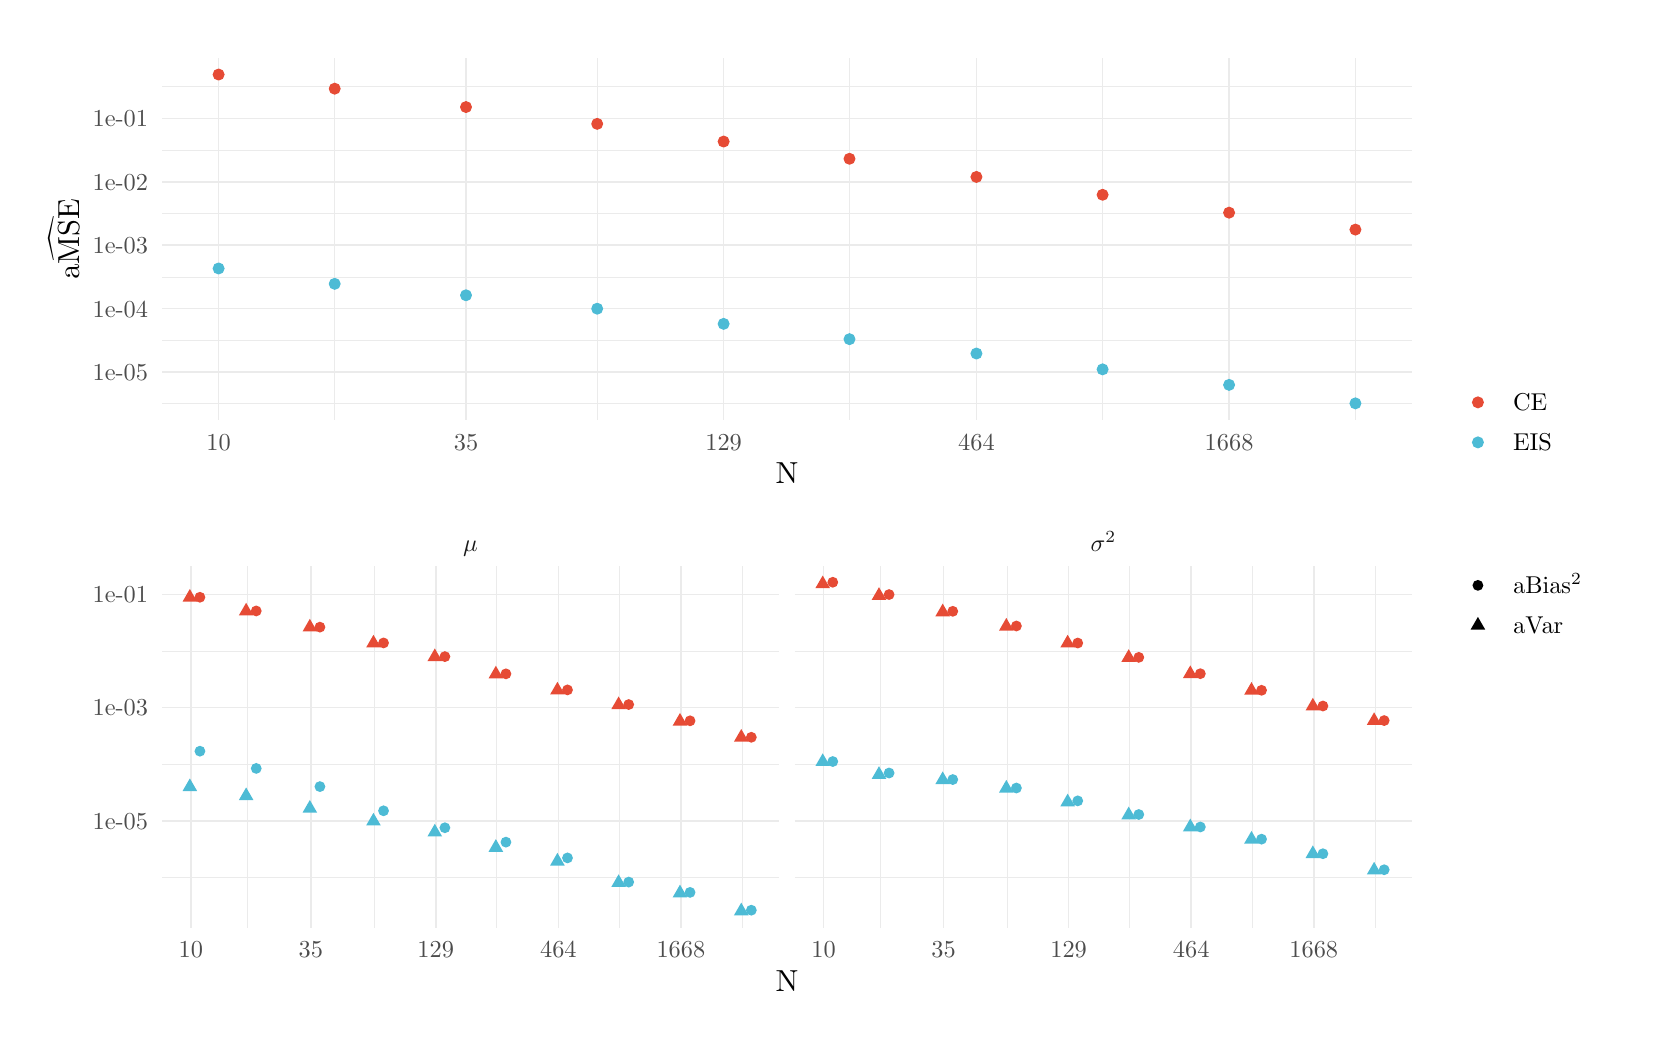
\begin{tikzpicture}[x=1pt,y=1pt]
\definecolor{fillColor}{RGB}{255,255,255}
\path[use as bounding box,fill=fillColor,fill opacity=0.00] (0,0) rectangle (578.16,361.35);
\begin{scope}
\path[clip] ( 48.45,219.65) rectangle (500.31,350.35);
\definecolor{drawColor}{gray}{0.92}

\path[draw=drawColor,line width= 0.3pt,line join=round] ( 48.45,225.46) --
	(500.31,225.46);

\path[draw=drawColor,line width= 0.3pt,line join=round] ( 48.45,248.36) --
	(500.31,248.36);

\path[draw=drawColor,line width= 0.3pt,line join=round] ( 48.45,271.25) --
	(500.31,271.25);

\path[draw=drawColor,line width= 0.3pt,line join=round] ( 48.45,294.15) --
	(500.31,294.15);

\path[draw=drawColor,line width= 0.3pt,line join=round] ( 48.45,317.04) --
	(500.31,317.04);

\path[draw=drawColor,line width= 0.3pt,line join=round] ( 48.45,339.94) --
	(500.31,339.94);

\path[draw=drawColor,line width= 0.3pt,line join=round] (110.94,219.65) --
	(110.94,350.35);

\path[draw=drawColor,line width= 0.3pt,line join=round] (205.79,219.65) --
	(205.79,350.35);

\path[draw=drawColor,line width= 0.3pt,line join=round] (296.96,219.65) --
	(296.96,350.35);

\path[draw=drawColor,line width= 0.3pt,line join=round] (388.42,219.65) --
	(388.42,350.35);

\path[draw=drawColor,line width= 0.3pt,line join=round] (479.78,219.65) --
	(479.78,350.35);

\path[draw=drawColor,line width= 0.6pt,line join=round] ( 48.45,236.91) --
	(500.31,236.91);

\path[draw=drawColor,line width= 0.6pt,line join=round] ( 48.45,259.81) --
	(500.31,259.81);

\path[draw=drawColor,line width= 0.6pt,line join=round] ( 48.45,282.70) --
	(500.31,282.70);

\path[draw=drawColor,line width= 0.6pt,line join=round] ( 48.45,305.60) --
	(500.31,305.60);

\path[draw=drawColor,line width= 0.6pt,line join=round] ( 48.45,328.49) --
	(500.31,328.49);

\path[draw=drawColor,line width= 0.6pt,line join=round] ( 68.99,219.65) --
	( 68.99,350.35);

\path[draw=drawColor,line width= 0.6pt,line join=round] (158.39,219.65) --
	(158.39,350.35);

\path[draw=drawColor,line width= 0.6pt,line join=round] (251.48,219.65) --
	(251.48,350.35);

\path[draw=drawColor,line width= 0.6pt,line join=round] (342.83,219.65) --
	(342.83,350.35);

\path[draw=drawColor,line width= 0.6pt,line join=round] (434.13,219.65) --
	(434.13,350.35);
\definecolor{drawColor}{RGB}{230,75,53}
\definecolor{fillColor}{RGB}{230,75,53}

\path[draw=drawColor,line width= 0.4pt,line join=round,line cap=round,fill=fillColor] ( 68.99,344.41) circle (  1.96);

\path[draw=drawColor,line width= 0.4pt,line join=round,line cap=round,fill=fillColor] (110.94,339.30) circle (  1.96);

\path[draw=drawColor,line width= 0.4pt,line join=round,line cap=round,fill=fillColor] (158.39,332.66) circle (  1.96);

\path[draw=drawColor,line width= 0.4pt,line join=round,line cap=round,fill=fillColor] (205.79,326.59) circle (  1.96);

\path[draw=drawColor,line width= 0.4pt,line join=round,line cap=round,fill=fillColor] (251.48,320.20) circle (  1.96);

\path[draw=drawColor,line width= 0.4pt,line join=round,line cap=round,fill=fillColor] (296.96,313.97) circle (  1.96);

\path[draw=drawColor,line width= 0.4pt,line join=round,line cap=round,fill=fillColor] (342.83,307.41) circle (  1.96);

\path[draw=drawColor,line width= 0.4pt,line join=round,line cap=round,fill=fillColor] (388.42,300.96) circle (  1.96);

\path[draw=drawColor,line width= 0.4pt,line join=round,line cap=round,fill=fillColor] (434.13,294.50) circle (  1.96);

\path[draw=drawColor,line width= 0.4pt,line join=round,line cap=round,fill=fillColor] (479.78,288.38) circle (  1.96);
\definecolor{drawColor}{RGB}{77,187,213}
\definecolor{fillColor}{RGB}{77,187,213}

\path[draw=drawColor,line width= 0.4pt,line join=round,line cap=round,fill=fillColor] ( 68.99,274.33) circle (  1.96);

\path[draw=drawColor,line width= 0.4pt,line join=round,line cap=round,fill=fillColor] (110.94,268.78) circle (  1.96);

\path[draw=drawColor,line width= 0.4pt,line join=round,line cap=round,fill=fillColor] (158.39,264.65) circle (  1.96);

\path[draw=drawColor,line width= 0.4pt,line join=round,line cap=round,fill=fillColor] (205.79,259.80) circle (  1.96);

\path[draw=drawColor,line width= 0.4pt,line join=round,line cap=round,fill=fillColor] (251.48,254.32) circle (  1.96);

\path[draw=drawColor,line width= 0.4pt,line join=round,line cap=round,fill=fillColor] (296.96,248.79) circle (  1.96);

\path[draw=drawColor,line width= 0.4pt,line join=round,line cap=round,fill=fillColor] (342.83,243.60) circle (  1.96);

\path[draw=drawColor,line width= 0.4pt,line join=round,line cap=round,fill=fillColor] (388.42,237.88) circle (  1.96);

\path[draw=drawColor,line width= 0.4pt,line join=round,line cap=round,fill=fillColor] (434.13,232.27) circle (  1.96);

\path[draw=drawColor,line width= 0.4pt,line join=round,line cap=round,fill=fillColor] (479.78,225.59) circle (  1.96);
\end{scope}
\begin{scope}
\path[clip] (  0.00,  0.00) rectangle (578.16,361.35);
\definecolor{drawColor}{gray}{0.30}

\node[text=drawColor,anchor=base east,inner sep=0pt, outer sep=0pt, scale=  0.88] at ( 43.50,233.88) {1e-05};

\node[text=drawColor,anchor=base east,inner sep=0pt, outer sep=0pt, scale=  0.88] at ( 43.50,256.78) {1e-04};

\node[text=drawColor,anchor=base east,inner sep=0pt, outer sep=0pt, scale=  0.88] at ( 43.50,279.67) {1e-03};

\node[text=drawColor,anchor=base east,inner sep=0pt, outer sep=0pt, scale=  0.88] at ( 43.50,302.57) {1e-02};

\node[text=drawColor,anchor=base east,inner sep=0pt, outer sep=0pt, scale=  0.88] at ( 43.50,325.46) {1e-01};
\end{scope}
\begin{scope}
\path[clip] (  0.00,  0.00) rectangle (578.16,361.35);
\definecolor{drawColor}{gray}{0.30}

\node[text=drawColor,anchor=base,inner sep=0pt, outer sep=0pt, scale=  0.88] at ( 68.99,208.64) {10};

\node[text=drawColor,anchor=base,inner sep=0pt, outer sep=0pt, scale=  0.88] at (158.39,208.64) {35};

\node[text=drawColor,anchor=base,inner sep=0pt, outer sep=0pt, scale=  0.88] at (251.48,208.64) {129};

\node[text=drawColor,anchor=base,inner sep=0pt, outer sep=0pt, scale=  0.88] at (342.83,208.64) {464};

\node[text=drawColor,anchor=base,inner sep=0pt, outer sep=0pt, scale=  0.88] at (434.13,208.64) {1668};
\end{scope}
\begin{scope}
\path[clip] (  0.00,  0.00) rectangle (578.16,361.35);
\definecolor{drawColor}{RGB}{0,0,0}

\node[text=drawColor,anchor=base,inner sep=0pt, outer sep=0pt, scale=  1.10] at (274.38,196.60) {N};
\end{scope}
\begin{scope}
\path[clip] (  0.00,  0.00) rectangle (578.16,361.35);
\definecolor{drawColor}{RGB}{0,0,0}

\node[text=drawColor,rotate= 90.00,anchor=base,inner sep=0pt, outer sep=0pt, scale=  1.10] at ( 18.58,285.00) {$\widehat{\mathrm{aMSE}}$};
\end{scope}
\begin{scope}
\path[clip] ( 48.45, 36.19) rectangle (271.63,166.89);
\definecolor{drawColor}{gray}{0.92}

\path[draw=drawColor,line width= 0.3pt,line join=round] ( 48.45, 54.35) --
	(271.63, 54.35);

\path[draw=drawColor,line width= 0.3pt,line join=round] ( 48.45, 95.22) --
	(271.63, 95.22);

\path[draw=drawColor,line width= 0.3pt,line join=round] ( 48.45,136.10) --
	(271.63,136.10);

\path[draw=drawColor,line width= 0.3pt,line join=round] ( 79.29, 36.19) --
	( 79.29,166.89);

\path[draw=drawColor,line width= 0.3pt,line join=round] (125.29, 36.19) --
	(125.29,166.89);

\path[draw=drawColor,line width= 0.3pt,line join=round] (169.52, 36.19) --
	(169.52,166.89);

\path[draw=drawColor,line width= 0.3pt,line join=round] (213.88, 36.19) --
	(213.88,166.89);

\path[draw=drawColor,line width= 0.3pt,line join=round] (258.19, 36.19) --
	(258.19,166.89);

\path[draw=drawColor,line width= 0.6pt,line join=round] ( 48.45, 74.78) --
	(271.63, 74.78);

\path[draw=drawColor,line width= 0.6pt,line join=round] ( 48.45,115.66) --
	(271.63,115.66);

\path[draw=drawColor,line width= 0.6pt,line join=round] ( 48.45,156.54) --
	(271.63,156.54);

\path[draw=drawColor,line width= 0.6pt,line join=round] ( 58.94, 36.19) --
	( 58.94,166.89);

\path[draw=drawColor,line width= 0.6pt,line join=round] (102.31, 36.19) --
	(102.31,166.89);

\path[draw=drawColor,line width= 0.6pt,line join=round] (147.46, 36.19) --
	(147.46,166.89);

\path[draw=drawColor,line width= 0.6pt,line join=round] (191.76, 36.19) --
	(191.76,166.89);

\path[draw=drawColor,line width= 0.6pt,line join=round] (236.05, 36.19) --
	(236.05,166.89);
\definecolor{fillColor}{RGB}{230,75,53}

\path[fill=fillColor] ( 62.24,155.53) circle (  1.96);

\path[fill=fillColor] ( 58.60,158.52) --
	( 61.24,153.94) --
	( 55.96,153.94) --
	cycle;
\definecolor{fillColor}{RGB}{77,187,213}

\path[fill=fillColor] ( 62.24, 99.91) circle (  1.96);

\path[fill=fillColor] ( 58.60, 90.07) --
	( 61.24, 85.50) --
	( 55.96, 85.50) --
	cycle;
\definecolor{fillColor}{RGB}{230,75,53}

\path[fill=fillColor] ( 82.59,150.58) circle (  1.96);

\path[fill=fillColor] ( 78.94,153.54) --
	( 81.59,148.96) --
	( 76.30,148.96) --
	cycle;
\definecolor{fillColor}{RGB}{77,187,213}

\path[fill=fillColor] ( 82.59, 93.68) circle (  1.96);

\path[fill=fillColor] ( 78.94, 86.81) --
	( 81.59, 82.23) --
	( 76.30, 82.23) --
	cycle;
\definecolor{fillColor}{RGB}{230,75,53}

\path[fill=fillColor] (105.60,144.73) circle (  1.96);

\path[fill=fillColor] (101.96,147.73) --
	(104.60,143.16) --
	( 99.32,143.16) --
	cycle;
\definecolor{fillColor}{RGB}{77,187,213}

\path[fill=fillColor] (105.60, 87.11) circle (  1.96);

\path[fill=fillColor] (101.96, 82.27) --
	(104.60, 77.69) --
	( 99.32, 77.69) --
	cycle;
\definecolor{fillColor}{RGB}{230,75,53}

\path[fill=fillColor] (128.59,139.02) circle (  1.96);

\path[fill=fillColor] (124.95,141.97) --
	(127.59,137.39) --
	(122.31,137.39) --
	cycle;
\definecolor{fillColor}{RGB}{77,187,213}

\path[fill=fillColor] (128.59, 78.37) circle (  1.96);

\path[fill=fillColor] (124.95, 77.65) --
	(127.59, 73.08) --
	(122.31, 73.08) --
	cycle;
\definecolor{fillColor}{RGB}{230,75,53}

\path[fill=fillColor] (150.76,134.08) circle (  1.96);

\path[fill=fillColor] (147.11,137.03) --
	(149.76,132.45) --
	(144.47,132.45) --
	cycle;
\definecolor{fillColor}{RGB}{77,187,213}

\path[fill=fillColor] (150.76, 72.24) circle (  1.96);

\path[fill=fillColor] (147.11, 73.68) --
	(149.76, 69.11) --
	(144.47, 69.11) --
	cycle;
\definecolor{fillColor}{RGB}{230,75,53}

\path[fill=fillColor] (172.82,127.85) circle (  1.96);

\path[fill=fillColor] (169.17,130.78) --
	(171.82,126.20) --
	(166.53,126.20) --
	cycle;
\definecolor{fillColor}{RGB}{77,187,213}

\path[fill=fillColor] (172.82, 67.04) circle (  1.96);

\path[fill=fillColor] (169.17, 68.14) --
	(171.82, 63.56) --
	(166.53, 63.56) --
	cycle;
\definecolor{fillColor}{RGB}{230,75,53}

\path[fill=fillColor] (195.06,122.05) circle (  1.96);

\path[fill=fillColor] (191.42,124.98) --
	(194.06,120.40) --
	(188.78,120.40) --
	cycle;
\definecolor{fillColor}{RGB}{77,187,213}

\path[fill=fillColor] (195.06, 61.34) circle (  1.96);

\path[fill=fillColor] (191.42, 63.18) --
	(194.06, 58.60) --
	(188.78, 58.60) --
	cycle;
\definecolor{fillColor}{RGB}{230,75,53}

\path[fill=fillColor] (217.18,116.76) circle (  1.96);

\path[fill=fillColor] (213.53,119.68) --
	(216.18,115.11) --
	(210.89,115.11) --
	cycle;
\definecolor{fillColor}{RGB}{77,187,213}

\path[fill=fillColor] (217.18, 52.61) circle (  1.96);

\path[fill=fillColor] (213.53, 55.43) --
	(216.18, 50.85) --
	(210.89, 50.85) --
	cycle;
\definecolor{fillColor}{RGB}{230,75,53}

\path[fill=fillColor] (239.35,110.88) circle (  1.96);

\path[fill=fillColor] (235.71,113.73) --
	(238.35,109.15) --
	(233.07,109.15) --
	cycle;
\definecolor{fillColor}{RGB}{77,187,213}

\path[fill=fillColor] (239.35, 48.88) circle (  1.96);

\path[fill=fillColor] (235.71, 51.68) --
	(238.35, 47.10) --
	(233.07, 47.10) --
	cycle;
\definecolor{fillColor}{RGB}{230,75,53}

\path[fill=fillColor] (261.49,104.93) circle (  1.96);

\path[fill=fillColor] (257.85,107.91) --
	(260.49,103.33) --
	(255.20,103.33) --
	cycle;
\definecolor{fillColor}{RGB}{77,187,213}

\path[fill=fillColor] (261.49, 42.45) circle (  1.96);

\path[fill=fillColor] (257.85, 45.18) --
	(260.49, 40.60) --
	(255.20, 40.60) --
	cycle;
\end{scope}
\begin{scope}
\path[clip] (277.13, 36.19) rectangle (500.31,166.89);
\definecolor{drawColor}{gray}{0.92}

\path[draw=drawColor,line width= 0.3pt,line join=round] (277.13, 54.35) --
	(500.31, 54.35);

\path[draw=drawColor,line width= 0.3pt,line join=round] (277.13, 95.22) --
	(500.31, 95.22);

\path[draw=drawColor,line width= 0.3pt,line join=round] (277.13,136.10) --
	(500.31,136.10);

\path[draw=drawColor,line width= 0.3pt,line join=round] (307.97, 36.19) --
	(307.97,166.89);

\path[draw=drawColor,line width= 0.3pt,line join=round] (353.97, 36.19) --
	(353.97,166.89);

\path[draw=drawColor,line width= 0.3pt,line join=round] (398.20, 36.19) --
	(398.20,166.89);

\path[draw=drawColor,line width= 0.3pt,line join=round] (442.56, 36.19) --
	(442.56,166.89);

\path[draw=drawColor,line width= 0.3pt,line join=round] (486.87, 36.19) --
	(486.87,166.89);

\path[draw=drawColor,line width= 0.6pt,line join=round] (277.13, 74.78) --
	(500.31, 74.78);

\path[draw=drawColor,line width= 0.6pt,line join=round] (277.13,115.66) --
	(500.31,115.66);

\path[draw=drawColor,line width= 0.6pt,line join=round] (277.13,156.54) --
	(500.31,156.54);

\path[draw=drawColor,line width= 0.6pt,line join=round] (287.62, 36.19) --
	(287.62,166.89);

\path[draw=drawColor,line width= 0.6pt,line join=round] (330.99, 36.19) --
	(330.99,166.89);

\path[draw=drawColor,line width= 0.6pt,line join=round] (376.14, 36.19) --
	(376.14,166.89);

\path[draw=drawColor,line width= 0.6pt,line join=round] (420.45, 36.19) --
	(420.45,166.89);

\path[draw=drawColor,line width= 0.6pt,line join=round] (464.73, 36.19) --
	(464.73,166.89);
\definecolor{fillColor}{RGB}{230,75,53}

\path[fill=fillColor] (290.92,160.95) circle (  1.96);

\path[fill=fillColor] (287.28,163.39) --
	(289.92,158.82) --
	(284.64,158.82) --
	cycle;
\definecolor{fillColor}{RGB}{77,187,213}

\path[fill=fillColor] (290.92, 96.17) circle (  1.96);

\path[fill=fillColor] (287.28, 99.14) --
	(289.92, 94.56) --
	(284.64, 94.56) --
	cycle;
\definecolor{fillColor}{RGB}{230,75,53}

\path[fill=fillColor] (311.27,156.50) circle (  1.96);

\path[fill=fillColor] (307.62,159.16) --
	(310.27,154.59) --
	(304.98,154.59) --
	cycle;
\definecolor{fillColor}{RGB}{77,187,213}

\path[fill=fillColor] (311.27, 92.02) circle (  1.96);

\path[fill=fillColor] (307.62, 94.48) --
	(310.27, 89.90) --
	(304.98, 89.90) --
	cycle;
\definecolor{fillColor}{RGB}{230,75,53}

\path[fill=fillColor] (334.28,150.45) circle (  1.96);

\path[fill=fillColor] (330.64,153.24) --
	(333.28,148.66) --
	(328.00,148.66) --
	cycle;
\definecolor{fillColor}{RGB}{77,187,213}

\path[fill=fillColor] (334.28, 89.66) circle (  1.96);

\path[fill=fillColor] (330.64, 92.60) --
	(333.28, 88.03) --
	(328.00, 88.03) --
	cycle;
\definecolor{fillColor}{RGB}{230,75,53}

\path[fill=fillColor] (357.27,145.14) circle (  1.96);

\path[fill=fillColor] (353.63,148.06) --
	(356.27,143.48) --
	(350.99,143.48) --
	cycle;
\definecolor{fillColor}{RGB}{77,187,213}

\path[fill=fillColor] (357.27, 86.60) circle (  1.96);

\path[fill=fillColor] (353.63, 89.53) --
	(356.27, 84.96) --
	(350.99, 84.96) --
	cycle;
\definecolor{fillColor}{RGB}{230,75,53}

\path[fill=fillColor] (379.44,138.99) circle (  1.96);

\path[fill=fillColor] (375.79,141.98) --
	(378.44,137.40) --
	(373.15,137.40) --
	cycle;
\definecolor{fillColor}{RGB}{77,187,213}

\path[fill=fillColor] (379.44, 81.96) circle (  1.96);

\path[fill=fillColor] (375.79, 84.57) --
	(378.44, 79.99) --
	(373.15, 79.99) --
	cycle;
\definecolor{fillColor}{RGB}{230,75,53}

\path[fill=fillColor] (401.50,133.81) circle (  1.96);

\path[fill=fillColor] (397.85,136.77) --
	(400.50,132.19) --
	(395.21,132.19) --
	cycle;
\definecolor{fillColor}{RGB}{77,187,213}

\path[fill=fillColor] (401.50, 77.03) circle (  1.96);

\path[fill=fillColor] (397.85, 79.89) --
	(400.50, 75.31) --
	(395.21, 75.31) --
	cycle;
\definecolor{fillColor}{RGB}{230,75,53}

\path[fill=fillColor] (423.74,127.91) circle (  1.96);

\path[fill=fillColor] (420.10,130.90) --
	(422.74,126.32) --
	(417.46,126.32) --
	cycle;
\definecolor{fillColor}{RGB}{77,187,213}

\path[fill=fillColor] (423.74, 72.52) circle (  1.96);

\path[fill=fillColor] (420.10, 75.55) --
	(422.74, 70.97) --
	(417.46, 70.97) --
	cycle;
\definecolor{fillColor}{RGB}{230,75,53}

\path[fill=fillColor] (445.86,121.91) circle (  1.96);

\path[fill=fillColor] (442.22,124.89) --
	(444.86,120.31) --
	(439.57,120.31) --
	cycle;
\definecolor{fillColor}{RGB}{77,187,213}

\path[fill=fillColor] (445.86, 68.12) circle (  1.96);

\path[fill=fillColor] (442.22, 71.10) --
	(444.86, 66.52) --
	(439.57, 66.52) --
	cycle;
\definecolor{fillColor}{RGB}{230,75,53}

\path[fill=fillColor] (468.03,116.23) circle (  1.96);

\path[fill=fillColor] (464.39,119.19) --
	(467.03,114.61) --
	(461.75,114.61) --
	cycle;
\definecolor{fillColor}{RGB}{77,187,213}

\path[fill=fillColor] (468.03, 62.85) circle (  1.96);

\path[fill=fillColor] (464.39, 65.87) --
	(467.03, 61.29) --
	(461.75, 61.29) --
	cycle;
\definecolor{fillColor}{RGB}{230,75,53}

\path[fill=fillColor] (490.17,110.97) circle (  1.96);

\path[fill=fillColor] (486.53,113.96) --
	(489.17,109.39) --
	(483.88,109.39) --
	cycle;
\definecolor{fillColor}{RGB}{77,187,213}

\path[fill=fillColor] (490.17, 57.06) circle (  1.96);

\path[fill=fillColor] (486.53, 59.93) --
	(489.17, 55.35) --
	(483.88, 55.35) --
	cycle;
\end{scope}
\begin{scope}
\path[clip] ( 48.45,166.89) rectangle (271.63,183.46);
\definecolor{drawColor}{gray}{0.10}

\node[text=drawColor,anchor=base,inner sep=0pt, outer sep=0pt, scale=  0.88] at (160.04,172.14) {$\mu$};
\end{scope}
\begin{scope}
\path[clip] (277.13,166.89) rectangle (500.31,183.46);
\definecolor{drawColor}{gray}{0.10}

\node[text=drawColor,anchor=base,inner sep=0pt, outer sep=0pt, scale=  0.88] at (388.72,172.14) {$\sigma^2$};
\end{scope}
\begin{scope}
\path[clip] (  0.00,  0.00) rectangle (578.16,361.35);
\definecolor{drawColor}{gray}{0.30}

\node[text=drawColor,anchor=base,inner sep=0pt, outer sep=0pt, scale=  0.88] at ( 58.94, 25.18) {10};

\node[text=drawColor,anchor=base,inner sep=0pt, outer sep=0pt, scale=  0.88] at (102.31, 25.18) {35};

\node[text=drawColor,anchor=base,inner sep=0pt, outer sep=0pt, scale=  0.88] at (147.46, 25.18) {129};

\node[text=drawColor,anchor=base,inner sep=0pt, outer sep=0pt, scale=  0.88] at (191.76, 25.18) {464};

\node[text=drawColor,anchor=base,inner sep=0pt, outer sep=0pt, scale=  0.88] at (236.05, 25.18) {1668};
\end{scope}
\begin{scope}
\path[clip] (  0.00,  0.00) rectangle (578.16,361.35);
\definecolor{drawColor}{gray}{0.30}

\node[text=drawColor,anchor=base,inner sep=0pt, outer sep=0pt, scale=  0.88] at (287.62, 25.18) {10};

\node[text=drawColor,anchor=base,inner sep=0pt, outer sep=0pt, scale=  0.88] at (330.99, 25.18) {35};

\node[text=drawColor,anchor=base,inner sep=0pt, outer sep=0pt, scale=  0.88] at (376.14, 25.18) {129};

\node[text=drawColor,anchor=base,inner sep=0pt, outer sep=0pt, scale=  0.88] at (420.45, 25.18) {464};

\node[text=drawColor,anchor=base,inner sep=0pt, outer sep=0pt, scale=  0.88] at (464.73, 25.18) {1668};
\end{scope}
\begin{scope}
\path[clip] (  0.00,  0.00) rectangle (578.16,361.35);
\definecolor{drawColor}{gray}{0.30}

\node[text=drawColor,anchor=base east,inner sep=0pt, outer sep=0pt, scale=  0.88] at ( 43.50, 71.75) {1e-05};

\node[text=drawColor,anchor=base east,inner sep=0pt, outer sep=0pt, scale=  0.88] at ( 43.50,112.63) {1e-03};

\node[text=drawColor,anchor=base east,inner sep=0pt, outer sep=0pt, scale=  0.88] at ( 43.50,153.51) {1e-01};
\end{scope}
\begin{scope}
\path[clip] (  0.00,  0.00) rectangle (578.16,361.35);
\definecolor{drawColor}{RGB}{0,0,0}

\node[text=drawColor,anchor=base,inner sep=0pt, outer sep=0pt, scale=  1.10] at (274.38, 13.14) {N};
\end{scope}
\begin{scope}
\path[clip] (  0.00,  0.00) rectangle (578.16,361.35);
\definecolor{drawColor}{RGB}{230,75,53}
\definecolor{fillColor}{RGB}{230,75,53}

\path[draw=drawColor,line width= 0.4pt,line join=round,line cap=round,fill=fillColor] (524.04,225.95) circle (  1.96);
\end{scope}
\begin{scope}
\path[clip] (  0.00,  0.00) rectangle (578.16,361.35);
\definecolor{drawColor}{RGB}{77,187,213}
\definecolor{fillColor}{RGB}{77,187,213}

\path[draw=drawColor,line width= 0.4pt,line join=round,line cap=round,fill=fillColor] (524.04,211.49) circle (  1.96);
\end{scope}
\begin{scope}
\path[clip] (  0.00,  0.00) rectangle (578.16,361.35);
\definecolor{drawColor}{RGB}{0,0,0}

\node[text=drawColor,anchor=base west,inner sep=0pt, outer sep=0pt, scale=  0.88] at (536.77,222.92) {CE};
\end{scope}
\begin{scope}
\path[clip] (  0.00,  0.00) rectangle (578.16,361.35);
\definecolor{drawColor}{RGB}{0,0,0}

\node[text=drawColor,anchor=base west,inner sep=0pt, outer sep=0pt, scale=  0.88] at (536.77,208.46) {EIS};
\end{scope}
\begin{scope}
\path[clip] (  0.00,  0.00) rectangle (578.16,361.35);
\definecolor{fillColor}{RGB}{0,0,0}

\path[fill=fillColor] (524.04,159.83) circle (  1.96);
\end{scope}
\begin{scope}
\path[clip] (  0.00,  0.00) rectangle (578.16,361.35);
\definecolor{fillColor}{RGB}{0,0,0}

\path[fill=fillColor] (524.04,148.42) --
	(526.68,143.85) --
	(521.40,143.85) --
	cycle;
\end{scope}
\begin{scope}
\path[clip] (  0.00,  0.00) rectangle (578.16,361.35);
\definecolor{drawColor}{RGB}{0,0,0}

\node[text=drawColor,anchor=base west,inner sep=0pt, outer sep=0pt, scale=  0.88] at (536.77,156.80) {aBias$^2$};
\end{scope}
\begin{scope}
\path[clip] (  0.00,  0.00) rectangle (578.16,361.35);
\definecolor{drawColor}{RGB}{0,0,0}

\node[text=drawColor,anchor=base west,inner sep=0pt, outer sep=0pt, scale=  0.88] at (536.77,142.34) {aVar};
\end{scope}
\end{tikzpicture}

    }
    \caption{{\color{red} TODO}}
    \label{fig:mse_bias_var_decomposition}
\end{figure}

% fig:mse_bias_var_decomposition
In \Cref{fig:mse_bias_var_decomposition} we see that the average MSE is much smaller for \acrshort{eis} compared to the 
\todo{interpretation of \Cref{fig:mse_bias_var_decomposition}, equal contribution of bias and var, not much to gain from bias correction}
\todo{is bias of CEM really of this order? would expect bias usually to be of order 1/n, bias squared of order 1/n squared, so negligible compared to 1/n mse?}
